\section{Modellbildung}


% Für jede Folie eine Frame-Umgebung erstellen
% Innerhalb der Frame-Umgebung werden dann die Inhalte geschrieben


\begin{frame}[fragile]
	\frametitle{Bild neben Bild}
		\begin{itemize}
			\item Beispieltstichpunkt Ebene 1
			\item Und noch ein Beispielstichpunkt
 		\end{itemize}

\begin{figure}[htbp]
        \centering

        \begin{subfigure}[b]{0.45\textwidth}
        		\centering
                
\includegraphics[width=\textwidth]{mechatronisches_antriebsystem.png} % relative width w.r.t. to the subfigure box
                \caption*{Struktur eines Antriebsystems}  % Hide label using \caption*{} instead of \caption
                \label{fig:myfigure2a}
        \end{subfigure}%
        \quad %add desired spacing between images, e. g. ~, \quad, \qquad, \hfill etc.
          %(or a blank line to force the subfigure onto a new line)
        \begin{subfigure}[b]{0.45\textwidth}
        		\centering
        		              
        		% You may insert \includegraphics here, but this is an example for tikz images:
        		\begin{externalize}
                \begin{tikzpicture}[align=center,auto]
	                % Tikz example adapted from http://www.texample.net/tikz/examples/tag/block-diagrams/
	                % Elemente
	                \tikzstyle{block} = [draw, rectangle, minimum height=1em, minimum width=2em]
	                \tikzstyle{sum} = [draw, circle]
	                \tikzstyle{every node}=[font=\tiny] % set fontsize for all nodes
	                
	                % Blöcke:
	                \node[coordinate] (input) {};
	                \node[sum] (sum) [right=0.4cm of input] {};
	                \node[block] (controller) [right=0.5cm of sum] {Controller};
	                \node[block] (system) [right=0.5cm of controller] {System};
	                \node[coordinate] (output) [right=0.6cm of system] {};
	                
	                % Verbindungen
	                \draw [->] (controller) -- node[name=u] {$u$} (system);
	                \draw [draw,->] (input) -- node {$w$} (sum);
	                \draw [->] (sum) -- node {$e$} (controller);
	                \draw [->] (system) -- node [name=y] {$y$}(output);
	                \draw [->] (y) |- ([yshift=-1em]system.south) -| node[pos=0.99] {$-$} node [near end] {$y_m$} (sum); %
                \end{tikzpicture}
                \end{externalize}
                \caption*{Allgemeine Reglerstruktur} % Hide label using \caption*{} instead of \caption
                \label{fig:myfigure2b}
        \end{subfigure}
        %\caption*{Blockschaltbilder}
        \label{fig:myfigure2}

	\begin{itemize}
		\item In den Abbildungen sieht man noch einmal den Unterschied zwischen Bitmaps (links) und Vektorgrafiken (rechts)
	\end{itemize}
\end{figure} 		
 		
\end{frame}



\begin{frame}{Zwei-Spalten Umgebung}


\begin{columns} % optional [c] or [T]
	\begin{column}{0.5\textwidth}
		Erste Spalte: 
		\begin{itemize}
			\item Nummer eins.
			\item Nummer zwei.
		\end{itemize}
	\end{column}
	\begin{column}{0.45\textwidth}
		Zweite Spalte:
		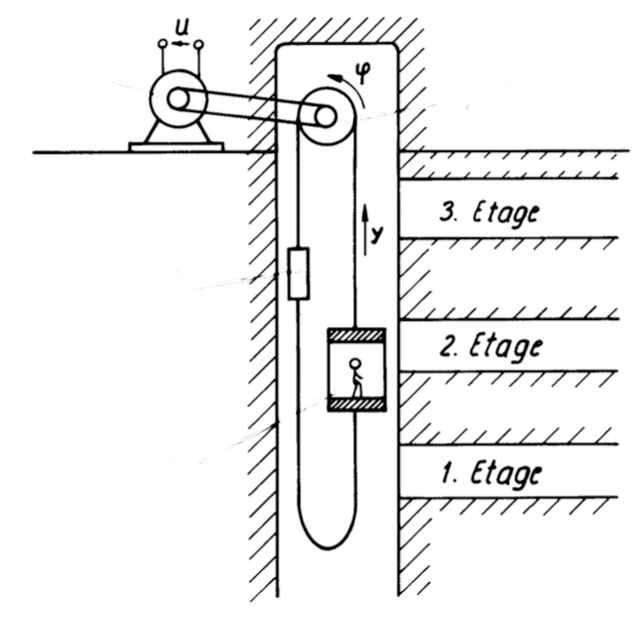
\includegraphics[width=0.9\columnwidth]{Aufzug.png}
	\end{column}
\end{columns}


\end{frame}

